\chapter{Test problems}

\section{Simulation problems}


\section{Control problems}
\subsection{Inverted pendulum}

\subsection{Tennessee Eastman challenge problem}
In 1993, \citet{downs.vogel1993plant-wide} proposed the Tennessee
Eastman plant-wide Industrial control problem as a test for new
control algorithms. The core of the process is a reactor with
a separation and recycle arrangement.  The flowsheet is shown in
Figure~\ref{fig:teprocess}.
\begin{figure}[htbp]
  \centering
  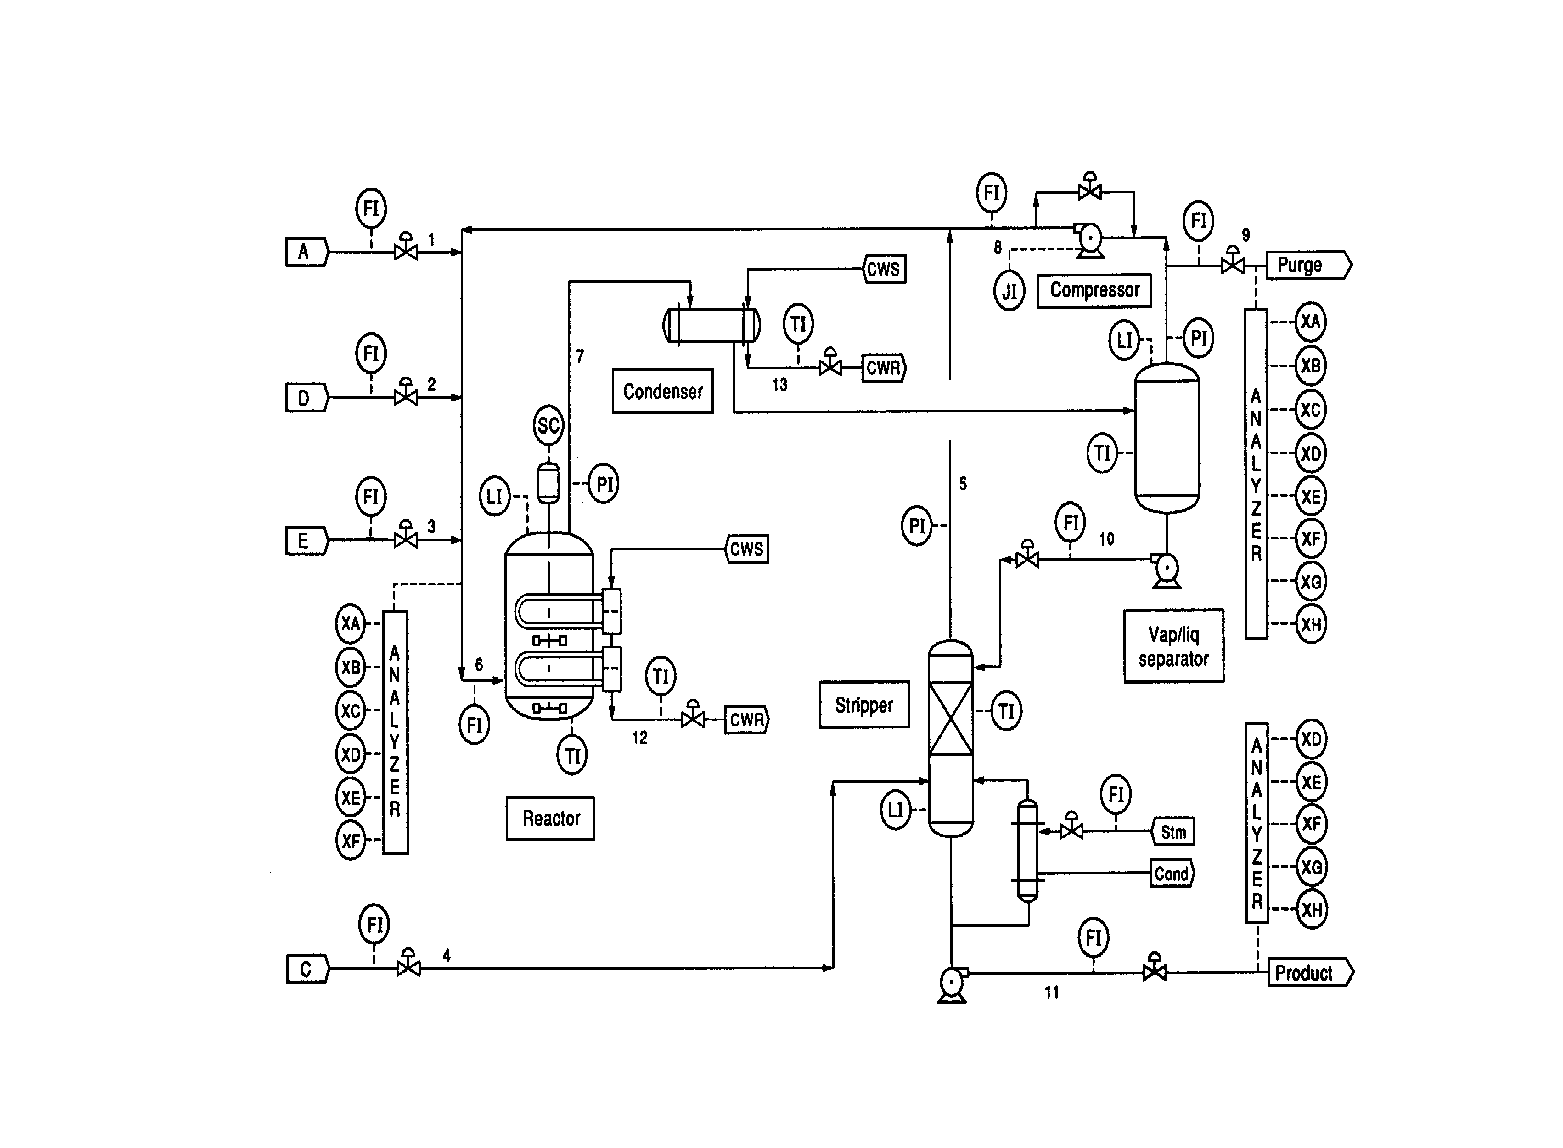
\includegraphics[width=\textwidth]{teflowsheet}
  \caption{Flowsheet for the Tennessee Eastman process~\citep{tenesseeeastman}}
  % TODO: Redraw TE flowsheet properly.
  \label{fig:teprocess}
\end{figure}

Four reactions featuring eight compounds (A through H) take place in the reactor:
\begin{eqnarray}
A(g) + C(g) + D(g) & \rightarrow & G(l) \\
A(g) + C(g) + E(g) & \rightarrow & H(l) \\
A(g) + E(g)        & \rightarrow & F(l) \\
3D(g)              & \rightarrow & 2F(l) 
\label{eq:te-reaction}
\end{eqnarray}

G and H are the first and second products, while F is a byproduct.


% Local Variables:
% TeX-master: "thesis"
% End:

